\documentclass[tikz,border=8pt]{standalone}
\usepackage{tikz}
\usetikzlibrary{arrows.meta,positioning,calc,fit}

\begin{document}
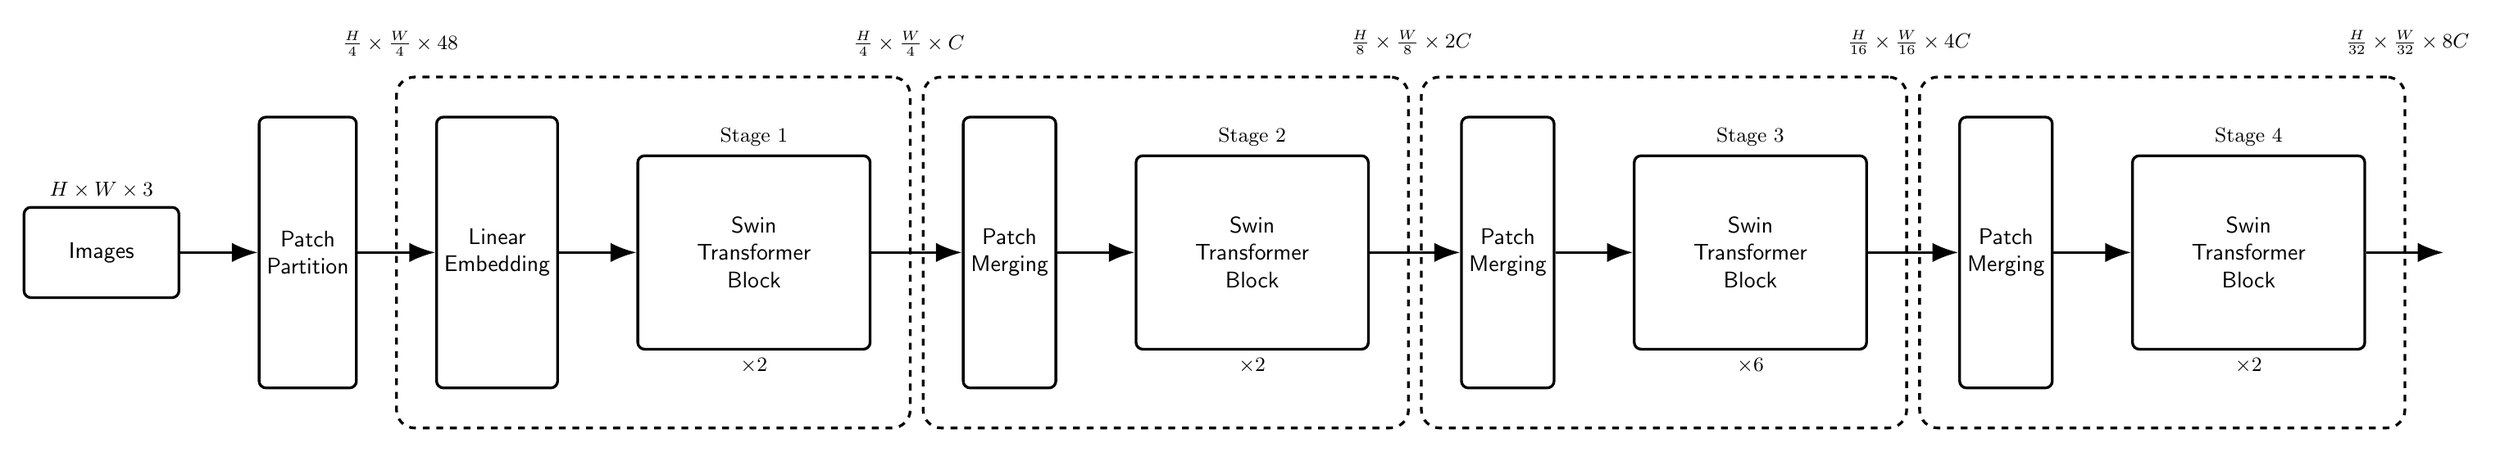
\begin{tikzpicture}[
  font=\sffamily,
  >={Latex[length=4mm,width=3mm]},
  line/.style={very thick, draw=black},
  box/.style={draw, very thick, rounded corners=3pt, align=center, fill=white},
  tall/.style={box, minimum width=14mm, minimum height=42mm},
  wide/.style={box, minimum width=36mm, minimum height=30mm},
  stageframe/.style={draw, very thick, rounded corners=8pt, dashed, inner sep=6mm},
  txt/.style={font=\small}
]

% ===== Left input =====
\node[box, minimum width=24mm, minimum height=14mm] (img) at (0,0) {Images};
\node[txt, anchor=south] at (img.north) {$H\times W\times 3$};

% Patch Partition (vertical)
\node[tall, right=12mm of img] (pp) {Patch\\Partition};

% Linear Embedding (vertical)
\node[tall, right=12mm of pp] (le) {Linear\\Embedding};

% Stage 1: Swin block
\node[wide, right=12mm of le] (s1) {Swin\\Transformer\\Block};
\node[txt, anchor=south] at (s1.north) {Stage 1};
\node[txt, anchor=north] at (s1.south) {$\times 2$};

% Stage 1 frame + top size
\node[stageframe, fit=(le)(s1)] (f1) {};
\node[txt, anchor=south] at ($(le.north)+(-15mm,8mm)$) {$\frac{H}{4}\times\frac{W}{4}\times 48$};

% Patch Merging between stages (vertical)
\node[tall, right=14mm of s1] (pm2) {Patch\\Merging};

% Stage 2
\node[wide, right=12mm of pm2] (s2) {Swin\\Transformer\\Block};
\node[txt, anchor=south] at (s2.north) {Stage 2};
\node[txt, anchor=north] at (s2.south) {$\times 2$};

\node[stageframe, fit=(pm2)(s2)] (f2) {};
\node[txt, anchor=south] at ($(f2.north)+(38mm,2mm)$) {$\frac{H}{8}\times\frac{W}{8}\times 2C$};

% Patch Merging to Stage 3
\node[tall, right=14mm of s2] (pm3) {Patch\\Merging};

% Stage 3
\node[wide, right=12mm of pm3] (s3) {Swin\\Transformer\\Block};
\node[txt, anchor=south] at (s3.north) {Stage 3};
\node[txt, anchor=north] at (s3.south) {$\times 6$};

\node[stageframe, fit=(pm3)(s3)] (f3) {};
\node[txt, anchor=south] at ($(f3.north)+(38mm,2mm)$) {$\frac{H}{16}\times\frac{W}{16}\times 4C$};

% Patch Merging to Stage 4
\node[tall, right=14mm of s3] (pm4) {Patch\\Merging};

% Stage 4
\node[wide, right=12mm of pm4] (s4) {Swin\\Transformer\\Block};
\node[txt, anchor=south] at (s4.north) {Stage 4};
\node[txt, anchor=north] at (s4.south) {$\times 2$};

\node[stageframe, fit=(pm4)(s4)] (f4) {};
\node[txt, anchor=south] at ($(f4.north)+(38mm,2mm)$) {$\frac{H}{32}\times\frac{W}{32}\times 8C$};

% ===== Arrows =====
\draw[line,->] (img.east) -- (pp.west);
\draw[line,->] (pp.east) -- (le.west);
\draw[line,->] (le.east) -- (s1.west);
\draw[line,->] (s1.east) -- (pm2.west);
\draw[line,->] (pm2.east) -- (s2.west);
\draw[line,->] (s2.east) -- (pm3.west);
\draw[line,->] (pm3.east) -- (s3.west);
\draw[line,->] (s3.east) -- (pm4.west);
\draw[line,->] (pm4.east) -- (s4.west);
\draw[line,->] (s4.east) -- ++(12mm,0);

% ===== Extra top label above Linear Embedding (as in figure) =====
\node[txt, anchor=south] at ($(s1.north)+(24mm,14mm)$) {$\frac{H}{4}\times\frac{W}{4}\times C$};

\end{tikzpicture}
\end{document}
